%-------------------------------------------------------------------------------
%
%     CHARGEMENT DES EXTENSIONS
%
%-------------------------------------------------------------------------------

\documentclass[11pt,fleqn]{report}
\usepackage{GarmirKhatch}

\definecolor{colone}{RGB}{209,220,204}
\definecolor{coltwo}{RGB}{204,222,210}
\definecolor{colthree}{RGB}{207,233,232}
\definecolor{colfour}{RGB}{248,243,214}
\definecolor{colfive}{RGB}{245,238,197}
\definecolor{colsix}{RGB}{243,235,179}
\definecolor{colseven}{RGB}{241,231,163}


%-------------------------------------------------------------------------------
%     Informations spécifiques au document
%-------------------------------------------------------------------------------

\ZTitle{Système de gestion des transports}
\ZSubject{Cahier des Charges Fonctionnel}
\ZVersion{2.3}
\ZDate{2014-03-09}

%-------------------------------------------------------------------------------
%     Contenu
%-------------------------------------------------------------------------------

\begin{document}

\ZMakeCover

\ZMakeInformations{
	% Historique des modifications
	% Version & Date & Auteur(s) & Modification(s)
	2.0 & 2014-03-03 & \Cadon & Création à partir de l'ancienne version \\
	\midrule
	2.1 & 2014-03-04 & \Pachy & Mise à jour en fonction de la réunion interne du 2014-03-03 \\
	\midrule
	2.2 & 2014-03-06 & \Lericolais & Mise à jour de la partie données \\
	\midrule
	2.3 & 2014-03-09 & \Cadon & Mise à jour corrective \\
}{
	% Historique des approbations
	% Version & Date & Approbateur(s)
	2.1 & 2014-03-09 & \Cadon \\
	\midrule
	2.3 & 2014-03-09 & \Cadon \\
}{
	% Historique des validations
	% Version & Date & Responsable(s)
	2.3 & 2014-03-21 & \Agopian \\
}

\ZMakeTableOfContents

\chapter{Présentation générale}

\section{Introduction}
Ce document constitue le cahier des charges du projet de \emph{système de gestion des transports} au bénéfice de la société \mo réalisé par l'assistance à maîtrise d'ouvrage \amo.

\section{\mo}

\subsection{Présentation}
Avec des dizaines de millions de volontaires dans 187 sociétés internationales, \mo est l'une des plus grandes organisations humanitaires au monde.
Elle agit avant, pendant et après les catastrophes et les urgences relatives à la santé pour répondre aux besoins des plus vulnérables et pour améliorer leur vie.
Elle dispense cette aide sans distinction de nationalité, de race, de religion, de classe ou d'opinions politiques.
\\
Elle puise sa force de son réseau de volontaires, de l'expertise basée dans la communauté et de sa capacité à donner une voix mondiale aux personnes vulnérables. Elle travaille en tant que partenaire dans le développement, la réponse aux catastrophes, l'aide pour une vie saine et sure, et l'amélioration des normes humanitaires. Le résultat : Elle aide à réduire les vulnérabilités, et rend les communautés plus résistantes.

\section{Contexte métier}
\mo possèdent des équipes de spécialistes formés aux interventions d'urgence dans le cadre notamment de catastrophes naturelles (tsunamis, tremblements de terre...).
Cinq domaines de compétence y sont représentés~:
\begin{itemize}
	\item médecine~;
	\item eau et sanitaire~;
	\item distribution~;
	\item logistique~;
	\item télécoms.
\end{itemize}
Leur dépendances respectives sont décrites dans la Figure \ref{dep}.
\begin{figure}[htbp]
	\centering
	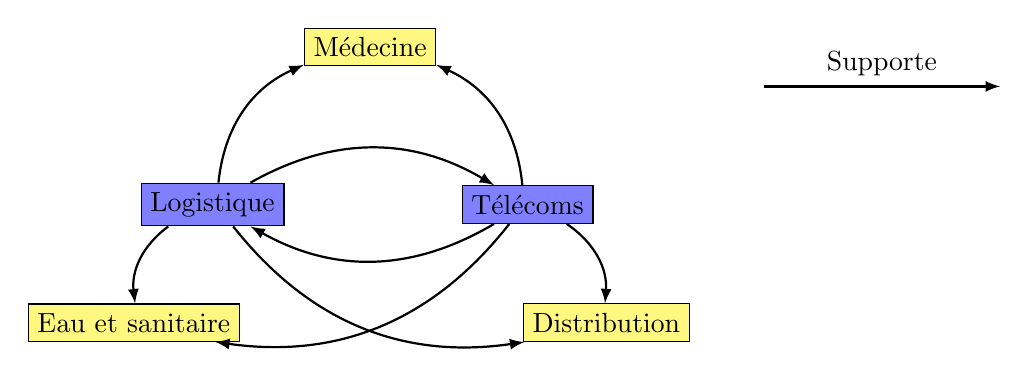
\begin{tikzpicture}
		% définition des styles
		\tikzstyle{metier}=[rectangle,draw,fill=yellow!50,text=black]
		\tikzstyle{support}=[rectangle,draw,fill=blue!50,text=black]
		\tikzstyle{supporte}=[->,>=latex,thick,rounded corners=4pt]
		% les nœuds
		\node[metier] (e) at (-3,-3) {Eau et sanitaire};
		\node[metier] (m) at (0,0.5) {Médecine};
		\node[metier] (d) at (3,-3) {Distribution};
		\node[support] (l) at (-2,-1.5) {Logistique};
		\node[support] (t) at (2,-1.5) {Télécoms};
		% les flèches
		\draw[supporte] (l) to[bend left] (t);
		\draw[supporte] (l) to[bend right] (e);
		\draw[supporte] (l) to[bend left] (m);
		\draw[supporte] (l) to[bend right] (d);
		\draw[supporte] (t) to[bend left] (l);
		\draw[supporte] (t) to[bend left] (e);
		\draw[supporte] (t) to[bend right] (m);
		\draw[supporte] (t) to[bend left] (d);
		% la légende
		\draw[supporte] (5,0) -- (8,0) node[midway,above]{Supporte};
	\end{tikzpicture}
	\caption{Dépendances entre les métiers}
	\label{dep}
\end{figure}

\subsubsection{La logistique}
L'efficacité de l'aide apportée aux populations sinistrées repose en particulier sur celle des processus logistiques.
De ce fait, la logistique apparaît comme un service support aux métiers (secteur médical, distribution, eau et sanitaires), sans lequel ils ne peuvent accomplir leurs missions.
\\
Actuellement, la logistique est confronté aux complications suivantes~:
\begin{itemize}
	\item la communication \& le partage d'informations sont peu efficaces~;
	\item les informations sont parfois redondantes~;
	\item les contraintes techniques \& environnementales~;
	\item la location de matériel donne lieu à la création de documents qui sont jusqu'à présent réalisés manuellement.
\end{itemize}

\paragraph{Processus et fonctions clefs de la logistique}
Différents processus concourent à l'accomplissement des missions logistiques dont~:
\begin{itemize}
	\item le processus d'achat~;
	\item le processus de stockage~;
	\item le processus de transport.
\end{itemize}
L'ensemble des processus doit permettre de répondre aux fonctions clefs de la logistique que sont notamment~:
\begin{itemize}
	\item planification/évaluation~;
	\item acquisition/achat~;
	\item organisation des transports~;
	\item gestion des entrepôts~;
	\item suivi et compte rendu~;
	\item standardisation~;
	\item formation et renforcement des capacités.
\end{itemize}

\paragraph{Les logisticiens de terrain}
En général, les équipes de logisticiens restent de dimension réduite (cinq à six personnes, dont un chef d'équipe), avec des profils spécialisés qui assurent en particulier des activités telles que~:
\begin{itemize}
	\item la mise en place et le maintien des procédures logistiques standards~;
	\item l'achat des biens et des services~;
	\item la facilitation de l'importation et de l'exportation des marchandises~;
	\item l'organisation du déploiement et du transport de la marchandise jusqu'aux sites de distribution~;
	\item l'organisation et la gestion des entrepôts~;
\end{itemize}
Chaque équipe reste déployée sur le terrain un mois (7j/7) et une mission d'urgence dure au plus quatre mois, délai au-delà duquel, la reconstruction prend le pas sur l'urgence.

\paragraph{Les transports}
Les transports occupent une place importante au sein de la chaîne logistique et répondent à deux grands types de services~:
\begin{itemize}
	\item le transport de personnes (les délégués)~;
	\item le transport de biens (NFI, ...).
\end{itemize}
Sauf cas exceptionnel, dans les premiers temps qui suivent une catastrophe, l'organisation ne dispose pas sur le terrain de ses propres moyens de transport de biens.
Les sociétés nationales de l'Organisation ne disposent pas en général non plus de ces moyens.
Il est alors du ressort de la logistique et en particulier du gestionnaire de flotte de trouver localement (entreprises privées, par exemple) les moyens de transport nécessaires (en général routiers).

\paragraph{Les outils}
Au cours du temps, avec l'expérience des catastrophes, l'Organisation a développé un certain nombre d'outils informatiques de terrain afin de l'aider dans ses tâches logistiques.
Parmi ces outils, figure notamment un logiciel qui permet aux équipes de disposer du suivi des biens dès lors que ceux-ci sont pris en charge au sein de la chaîne logistique sur le terrain et qui permet notamment de faciliter la traçabilité nécessaire afin de répondre aux attentes des parties prenantes, comme les donateurs notamment.

\section{Objectifs}

\subsection{Finalités}
Le but du projet est d'offrir une solution de type Transport~Management~System (appelé ci-après TMS) afin d'optimiser les ressources logistiques.
Grâce au TMS, \mo espère améliorer la qualité de ses services en se dotant d'un outil permettant de~:
\begin{itemize}
	\item \emph{planifier} les trajets, les chargements et déchargements, les dates de livraison~;
	\item \emph{réaliser} les opérations logistiques en temps voulu~;
	\item \emph{suivre} les transports et ainsi produire des documents synthétisant l'ensemble d'un trajet ou d'une cargaison~;
	\item \emph{améliorer} les processus existants grâce (entre autres) à l'établissement de statistiques permettant une mesure de l'efficience.
\end{itemize}
\mo espère ainsi, grâce à l'assistance de l'outil et l'automatisation de certaines de ces tâches, améliorer le fonctionnement global de l'organisation en suivant la logique décrite dans la Figure \ref{arbre_probleme}.

\subsection{Espérance de retour sur investissement}
\mo espère que le TMS lui permettra non seulement de réduire les coûts relatifs à la logistique mais également de maintenir son professionnalisme, améliorant ainsi son image de marque par preuve de son efficacité et de son efficience sur le terrain.
\begin{figure}[htbp] % Arbre à problèmes
	\centering
	\begin{tikzpicture} [
			node distance = 1cm, auto,font=\footnotesize,
			% STYLES
			every node/.style={node distance=3cm},
			% The comment style is used to describe the characteristics of each force
			comment/.style={rectangle, inner sep= 5pt, text width=4cm, node distance=0.25cm, font=\scriptsize\sffamily},
			% The force style is used to draw the forces' name
			force/.style={rectangle, draw, fill=black!10, inner sep=5pt, text width=4cm, text badly centered, minimum height=1.2cm, font=\bfseries\normalsize\sffamily}
		] 
		% Nodes
		\node [force] (confiance) {Confiance\\{\normalfont\footnotesize Envers \mo}};
		\node [force, above of=confiance] (transparent) {Transparence des informations\\{\normalfont\footnotesize Grâce au suivi détaillé}};
		%% Mj %% Bug avec 'X[cm] of transparent' -> Mise ne commentaire et réécriture sans
		\node [force, right=1cm of transparent] (serieux) {Sérieux\\{\normalfont\footnotesize Car on peut justifier à tout moment de l'utilisation des ressources}};
		\node [force, left=1cm of transparent] (pro) {Professionnalisme\\{\normalfont\footnotesize Notamment grâce à la planification et à l'utilisation optimale du matériel}};
		\node [force, below of=confiance, left=-1cm of confiance] (don) {Dons à l'organisation};
		\node [force, below of=confiance, right=-1cm of confiance] (benevolat) {Hausse du bénévolat};
%		\node [force, right] (serieux) {Sérieux\\{\normalfont\footnotesize Car on peut justifier à tout moment de l'utilisation des ressources}};
%		\node [force, left] (pro) {Professionnalisme\\{\normalfont\footnotesize Notamment grâce à la planification et à l'utilisation optimale du matériel}};
%		\node [force, below of=confiance, left] (don) {Dons à l'organisation};
%		\node [force, below of=confiance, right] (benevolat) {Hausse du bénévolat};
		% Draw the links between forces
		\path[->,thick]
			(don) edge (confiance)
			(benevolat) edge (confiance)
			(confiance) edge (transparent)
			(confiance) edge (serieux)
			(confiance) edge (pro);
		\end{tikzpicture} 
	\caption{Arbre à problème~: finalité du projet et retour sur investissement}
	\label{arbre_probleme}
\end{figure}

\section{Contexte de réalisation}

\subsection{Études déjà effectuées}
Une étude des scenarii possibles quant aux possibilités de l'organisation de se doter d'une solution logicielle adéquate a montré que les produits présents sur le marché ne répondaient qu'imparfaitement aux attentes de l'Organisation~:
\begin{itemize}
	\item inadéquation des solutions à certaines contraintes spécifiques du contexte d'urgence (moyens de communication à haut débit déficients...)~;
	\item solutions propriétaires~;
	\item solutions trop complexes~;
	\item solutions onéreuses.
\end{itemize}
Le scénario retenu est de fait celui d'un développement spécifique (basé éventuellement sur un noyau public) dont les fonctionnalités pourraient s'enrichir au cours du temps, avec des investissements progressifs.

\subsection{Nature des prestations demandées}
\mo cherche donc un prestataire pour la réalisation d'une solution complète de type TMS qui devra s'intégrer sans perturber le bon fonctionnement des processus existants. La solution pourra être basée sur un noyau public existant.
\\
Les prestations attendues sont~:
\begin{itemize}
	\item la suite logicielle~;
	\item le matériel (si nécessaire)~;
	\item le service support.
\end{itemize}

\subsection{Situation du projet par rapport aux autres projets de l'Organisation}
Ce projet s'intégrant à une infrastructure informatique déjà existante, cette partie tient compte des autres projets menés en parallèles et susceptibles d'impacter sur celui-ci.

\subsubsection{Migration des serveurs}
Une migration des serveurs de \mo est actuellement en projet.
Il s'agirait de migrer d'un environnement Microsoft~Windows actuellement en place, vers une distribution GNU/Linux dont le détail n'est pas encore connu.
Aucune date n'a encore été arrêtée.

\subsection{Suites prévues}
Les évolutions futures pourront être~:
\begin{itemize}
	\item ajout de fonctionnalités pour l'intégration de diverses composantes métier de \mo~;
	\item portage sur d'autres systèmes d'exploitation~;
	\item ...
\end{itemize}

\subsection{Parties concernées}

\subsubsection{Directement}
Les logisticiens de \mo en seront les principaux utilisateurs.
Le secrétariat central, par exemple, assurera le suivi de l'ensemble de la logistique à l'aide de cet outil.
Les métiers auront également accès aux informations relatives au matériel attendu ou à livrer.

\subsubsection{Indirectement}
Le temps gagné grâce à la solution permettra un acheminement plus rapide des marchandises, denrées, et personnels~; ce temps est crucial en situation d'urgence.
L'économie réalisée permettra d'augmenter les capacités, et les moyens d'action de l'association dans ses activités.
\\
Les victimes prises en charge seront donc indirectement bénéficiaires.

\subsection{Caractère confidentiel s'il y a lieu}
\mo se rapproche d'une autre association par ses activités métier et son mode de fonctionnement.
Bien que cette autre association puisse bénéficier de ce projet, il conviendra de ne pas faire de rapprochement avec celle-ci tant que sa participation au projet ne sera pas officiellement engagée.

\section{Énoncé du besoin}
Il est attendu de la solution qu'elle fonctionne sur l'architecture générale présentée dans la figure \ref{ArchitectureGenerale}.
\begin{figure}[htbp]
	\centering
	\begin{tikzpicture}
		% Définition des styles
		\tikzstyle{sup} = [rectangle,draw=white,text=black,text centered,minimum width=20mm,minimum height=80mm]
		\tikzstyle{one} = [fill=colone,rectangle,draw=white,minimum width=20mm]
		\tikzstyle{two} = [fill=coltwo,rectangle,draw=white,minimum width=20mm]
		\tikzstyle{three} = [fill=colthree,rectangle,draw=white,minimum width=20mm]
		\tikzstyle{four} = [fill=colfour,rectangle,draw=white,minimum width=20mm]
		\tikzstyle{five} = [fill=colfive,rectangle,draw=white,minimum width=20mm]
		\tikzstyle{six} = [fill=colsix,rectangle,draw=white,minimum width=20mm]
		\tikzstyle{seven} = [fill=colseven,rectangle,draw=white,minimum width=20mm]
		\tikzstyle{inf} = [rectangle,draw=white,text=black,text centered,minimum width=20mm,minimum height=10mm]
		\tikzstyle{oneonthree} = [minimum height=26mm]
		\tikzstyle{twoonthree} = [minimum height=28mm]
		\tikzstyle{threeonthree} = [minimum height=26mm]
		\tikzstyle{oneonfour} = [minimum height=20mm]
		\tikzstyle{twoonfour} = [minimum height=20mm]
		\tikzstyle{threeonfour} = [minimum height=20mm]
		\tikzstyle{fouronfour} = [minimum height=20mm]
		\tikzstyle{arrow}=[->,>=latex,thick,rounded corners=4pt]
		% Noeuds utilisateurs
		\node[inf,one] at (  0mm, 0mm) {\centering\tiny\bfseries\scshape Utilisateurs};
		\node[one,oneonthree] (Utilisateurs) at (  0mm,18mm) {};
		\node at (  0mm,9mm) {\centering\tiny\itshape Métier};
		\node at (  0mm,19mm) {\centering\includegraphics[height=16mm]{"Logistician"}};
		\node[one,twoonthree] (Logistician) at (  0mm,45mm) {};
		\node at (  0mm,36mm) {\centering\tiny\itshape Logisticien};
		\node at (  0mm,46mm) {\centering\includegraphics[height=16mm]{"Logistician"}};
		\node[one,threeonthree] (Administrateur) at (  0mm,72mm) {};
		\node at (  0mm,63mm) {\centering\tiny\itshape Administrateur};
		\node at (  0mm,73mm) {\centering\includegraphics[height=16mm]{"Logistician"}};
		% Noeuds matériels
		\node[inf,two] at ( 20mm, 0mm) {\centering\tiny\bfseries\scshape Matériels};
		\node[two,oneonthree] (Matériels) at ( 20mm,18mm) {};
		\node at ( 20mm,9mm) {\centering\tiny\itshape Portable};
		\node at ( 20mm,19mm) {\centering\includegraphics[width=16mm]{"Laptop computer"}};
		\node[two,twoonthree] (Smartphone) at ( 20mm,45mm) {};
		\node at ( 20mm,36mm) {\centering\tiny\itshape Smartphone};
		\node at ( 20mm,46mm) {\centering\includegraphics[height=16mm]{"Smartphone"}};
		\node[two,threeonthree] (Satphone) at ( 20mm,72mm) {};
		\node at ( 20mm,63mm) {\centering\tiny\itshape Téléphone satellite};
		\node at ( 20mm,73mm) {\centering\includegraphics[height=16mm]{"Smartphone"}};
		% Noeuds application
		\node[inf,three] at ( 40mm, 0mm) {\centering\tiny\bfseries\scshape Application(s)};
		\node[three,minimum width=20mm,minimum height=80mm] (Application) at ( 40mm,45mm) {\centering};
		% Noeuds synchronisation
		\node[inf,four] at ( 60mm, 0mm) {\centering\tiny\bfseries\scshape Synchro};
		\node[four,oneonfour] (Physique1) at ( 60mm,15mm) {};
		\node at ( 60mm, 9mm) {\centering\tiny\itshape Physique};
		\node at ( 56mm,16mm) {\centering\includegraphics[width=6mm]{"Compact disk"}};
		\node at ( 64mm,16mm) {\centering\includegraphics[width=8mm]{"USB key"}};
		\node[four,twoonfour] (Internet1) at ( 60mm,35mm) {};
		\node at ( 60mm,29mm) {\centering\tiny\itshape Internet};
		\node at ( 60mm,36mm) {\centering\includegraphics[width=16mm]{"Internet"}};
		\node[four,threeonfour] (Téléphonie1) at ( 60mm,55mm) {};
		\node at ( 60mm,49mm) {\centering\tiny\itshape Téléphonie};
		\node at ( 60mm,56mm) {\centering\includegraphics[height=16mm]{"Phone antenna"}};
		\node[four,fouronfour] (Satellite1) at ( 60mm,75mm) {};
		\node at ( 60mm,69mm) {\centering\tiny\itshape Satellite};
		\node at ( 60mm,76mm) {\centering\includegraphics[height=16mm]{"Satellite"}};
		% Noeuds serveur local
		\node[inf,five] at ( 80mm, 0mm) {\centering\tiny\bfseries\scshape\begin{tabular}{c}Serveur \\ local\end{tabular}};
		\node[five,minimum height=80mm] (Server1) at (80mm,45mm) {};
		\node at (80mm,34mm) {\centering\tiny\itshape Serveur};
		\node at (80mm,48mm) {\centering\includegraphics[width=16mm]{"Server"}};
		% Noeuds synchronisation
		\node[inf,six] at (100mm, 0mm) {\centering\tiny\bfseries\scshape Synchro};
		\node[six,oneonfour] (Physique1) at (100mm,15mm) {};
		\node at (100mm, 9mm) {\centering\tiny\itshape Physique};
		\node at ( 96mm,16mm) {\centering\includegraphics[width=6mm]{"Compact disk"}};
		\node at (104mm,16mm) {\centering\includegraphics[width=8mm]{"USB key"}};
		\node[six,twoonfour] (Internet2) at (100mm,35mm) {};
		\node at (100mm,29mm) {\centering\tiny\itshape Internet};
		\node at (100mm,36mm) {\centering\includegraphics[width=16mm]{"Internet"}};
		\node[six,threeonfour] (Téléphonie2) at (100mm,55mm) {};
		\node at (100mm,49mm) {\centering\tiny\itshape Téléphonie};
		\node at (100mm,56mm) {\centering\includegraphics[height=16mm]{"Phone antenna"}};
		\node[six,fouronfour] (Satellite2) at (100mm,75mm) {};
		\node at (100mm,69mm) {\centering\tiny\itshape Satellite};
		\node at (100mm,76mm) {\centering\includegraphics[height=16mm]{"Satellite"}};
		% Noeuds serveur central
		\node[inf,seven] at (120mm, 0mm) {\centering\tiny\bfseries\scshape\begin{tabular}{c}Serveur \\ central\end{tabular}};
		\node[seven,minimum height=80mm] (Server2) at (120mm,45mm) {};
		\node at (120mm,34mm) {\centering\tiny\itshape Serveur};
		\node at (120mm,48mm) {\centering\includegraphics[width=16mm]{"Server"}};
		\end{tikzpicture}
	\caption{Architecture générale}
	\label{ArchitectureGenerale}
\end{figure}

\label{liste_exhaustive_elts_contraintes}
\subsection{Utilisateurs}
De nombreux utilisateurs de différents types seront amenés à utiliser la suite logicielle.
Ces derniers seront principalement~:
\begin{itemize}
	\item le secrétariat central~;
	\item les logisticiens de terrain~;
	\item les métiers~;
	\item les administrateurs~;
\end{itemize}

\subsection{Matériels}
\mo possède déjà de nombreux matériels normalisés décris ci-dessous.
Parmi ces derniers, il est attendu que la suite logicielle soit pleinement accessible depuis ordinateurs portables, smartphones et téléphones satellite.
\mo dispose~:
\begin{itemize}
	\item de serveurs (locaux et central) actuellement sous Microsoft~Windows (une migration vers une distribution GNU/Linux étant en projet).
		Le stockage actuel des données est pris en charge par deux SGBDR que sont MySQL~Server et SQL~Oracle~;
	\item d'ordinateurs portables sous Microsoft~Windows~7.
		Ils sont équipés de 16 Go de mémoire vive et de 250 Go d'espace disque.
		\href{https://www.microsoft.com/fr-fr/download/internet-explorer.aspx}{Microsoft~Internet~Explorer~11} et \href{http://www.mozilla.org/en-US/firefox/27.0.1/releasenotes/}{Mozilla~Firefox~27.0.1} sont les deux navigateurs présents par défaut et leur utilisation est fonction des préférences de l'utilisateur~;
	\item de terminaux satellitaires \href{http://explorersatellite.com/BGAN/thrane_thrane_bgan.html}{BGAN (Thrane \& Thrane~Explorer~500)}~;
	\item de smartphones sous \href{http://www.android.com/}{Android}~;
	\item de téléphones satellitaires Thuraya (\href{http://www.thuraya.com.kw/hughes7101.html}{Hughes~7100} / \href{http://www.thuraya.com.kw/hughes7100.html}{7101} et \href{http://www.thuraya.com.kw/so-2510.html}{SO~2510}) et Iridium (\href{http://www.iridium.com/products/Iridium-9505A-Satellite-Phone.aspx}{9505A} et \href{http://www.iridium.com/products/Iridium9555SatellitePhone.aspx}{9555}) destinés principalement à la communication vocale~;
	\item de téléphones télécopieurs (fax) satellitaires (Nera~Mini-M~Worldphone)~;
	\item de communicateurs radio VHF (Motorola~GP360/GM360)~;
	\item de points d'accès sans fil (Linksys~WRT54G) permettant de partager une connexion à large bande (BGAN, ADSL, VSAT, etc.) dans un réseau sans fil~;
	\item de GPS portables (eTrex~Venture~HC de Garmin).
\end{itemize}
\begin{constraint}[Contrainte de compatibilité]
	La suite logicielle doit impérativement être compatible avec les matériels énoncés.
	En outre, elle doit également être compatible avec les systèmes d'exploitation et, au minimum, les versions de logiciels précisés (un support pour versions ultérieurs pouvant être sollicité).
\end{constraint}
\begin{constraint}[Contrainte de coûts de communication]
	Bien que l'Organisation dispose de nombreux moyens de communications satellitaires, ces derniers sont principalement destinés aux urgences, car extrêmement coûteux.
	Un besoin fondamental est donc de minimiser ce genre de transferts, ainsi que d'avertir un utilisateur sur le point d'y avoir recours, afin de prévenir les cas d'erreur ou d'inattention.
	La priorité sur les moyens de communication utilisés devraient se plier aux préférences suivantes (par ordre décroissant)~:
	\begin{enumerate}
		\item les réseaux Internet~;
		\item les réseaux GSM~;
		\item les transports physiques~;
		\item les réseaux satellitaires.
	\end{enumerate}
\end{constraint}

\subsection{Application}
Le TMS doit~:
\begin{itemize}
	\item permettre une planification \& un suivi des transports~;
	\item être multilingue~;
	\item avoir des interfaces utilisateurs personnalisées dépendant de la fonction de l'utilisateur~;
	\item mémoriser les préférences utilisateur (e.g. la langue de l'application)~;
	\item gérer explicitement la sécurité des communications~;
	\item authentifier les utilisateurs (si le contexte d'utilisation le permet)~;
	\item gérer les sauvegardes et être compatible avec les grandes solutions du marché~;
	\item gérer explicitement la synchronisation, les importations, et les exportations de données autant entre les clients et le serveur local qu'entre le serveur local et le serveur central (dans les cas où les moyens de communications sont réduits)~;
	\item produire des documents de synthèse (i.e. tableaux de bord) dont le contenu est personnalisable en fonction du destinataire~;
	\item gérer les documents internes (réquisitions, waybills/delivery notes, ...)~;
	\item gérer les documents externes (contrats, patentes, ...)~;
	\item produire des statistiques personnalisables.
\end{itemize}

\chapter{Expression fonctionnelle du besoin}

\section{Fonctions de service et de contrainte}
Cette section précise les services attendus et contraintes à respecter.
\\
Il est attendu de la suite logicielle qu'elle réponde à l'architecture de la figure \ref{ArchitectureGenerale}.
Les fonctionnalité qui ne sont pas suivies d'une note de fonctionnalité complémentaire sont partie intégrante des services principaux attendus.
Ces derniers sont la raison d'être du produit et donc incontournables.

\subsection{La localisation}
La suite logicielle doit proposer des versions traduites en plusieurs langues, y compris avec des alphabets et des sens de lecture différents.
Au minimum, les traductions dans les langages suivants doivent être fournis~:
\begin{itemize}
	\item Anglais~;
	\item Arabe~;
	\item Espagnol~;
	\item Français.
\end{itemize}
En outre, la solution doit permettre de passer \emph{aisément} d'une langue à l'autre sans nécessiter de redémarrage.

\subsection{L'interface utilisateur}
La solution doit fournir au minimum et pour chacun de ces groupes utilisateurs une interface propre permettant de réaliser les actions suivantes~:
\begin{itemize}
	\item gestionnaire de transport~:
	\begin{itemize}
		\item moyen de contrôle des opérations (à venir, en cours...),
		\item outil d'édition de tableaux de bord~;
	\end{itemize}
	\item gestionnaire de la planification~:
	\begin{itemize}
		\item fournir aux métiers des données relatives à l'état des transports en cours~;
	\end{itemize}
	\item gestionnaire des prestataires~:
	\begin{itemize}
		\item édition de bons pour accord de paiement~;
	\end{itemize}
	\item métiers~:
	\begin{itemize}
		\item consultation des transports en cours en relation avec le métier~;
	\end{itemize}
	\item secrétariat central~:
	\begin{itemize}
		\item accès aux documents sous forme numérique,
		\item statistiques.
	\end{itemize}
\end{itemize}

\subsection{Les cas d'utilisations}
Cette section présente le diagramme des cas d'utilisation et précise pour chacun d'eux l'ensemble des actions attendues.
\begin{figure}[htbp]
	\begin{tikzpicture}
		\begin{umlsystem}[x=8.00,y=11.00,fill=red!10]{Administration}
			\umlusecase[x=0.00,y=0.00,name=GSauvegarde]{Gestion des sauvegardes}
			\umlusecase[x=0.00,y=1.00,name=GDroits]{Gestion des droits d'accès}
			\umlusecase[x=0.00,y=2.00,name=GSécurité]{Gestion des niveaux de sécurité (cryptographie)}
		\end{umlsystem}
		\begin{umlsystem}[x=8.00,y=0.00,fill=green!10]{Gestion des ressources}
			\umlusecase[x=0.00,y=0.00,name=GPrestataires]{Gestion des prestataires}
			\umlusecase[x=0.00,y=1.00,name=GTransports]{Gestion des moyens de transport}
			\umlusecase[x=0.00,y=2.00,name=GChauffeurs]{Gestion des chauffeurs}
			\umlusecase[x=0.00,y=3.00,name=GRéquisitions]{Gestion des réquisitions}
			\umlusecase[x=0.00,y=4.00,name=GWaybills]{Gestion des waybills/delivery~notes}
			\umlusecase[x=0.00,y=5.00,name=GTableauxBord]{Gestion des tableaux de bord}
			\umlusecase[x=0.00,y=6.00,name=GStatistiques]{Gestion des statistiques}
			\umlusecase[x=0.00,y=7.00,name=GSynchronisation]{Gestion de la synchronisation}
			\umlusecase[x=0.00,y=8.00,name=GPréférences]{Gestion des préférences}
		\end{umlsystem}
		\umlactor[x=0.00,y=10.00]{Administrateur}
		\umlactor[x=0.00,y=3.00]{Utilisateur}
		\umlinherit{Administrateur}{Utilisateur}
		\umlassoc{Utilisateur}{GPrestataires}
		\umlassoc{Utilisateur}{GTransports}
		\umlassoc{Utilisateur}{GChauffeurs}
		\umlassoc{Utilisateur}{GRéquisitions}
		\umlassoc{Utilisateur}{GWaybills}
		\umlassoc{Utilisateur}{GTableauxBord}
		\umlassoc{Utilisateur}{GStatistiques}
		\umlassoc{Utilisateur}{GSynchronisation}
		\umlassoc{Utilisateur}{GPréférences}
		\umlassoc{Administrateur}{GSauvegarde}
		\umlassoc{Administrateur}{GDroits}
		\umlassoc{Administrateur}{GSécurité}
	\end{tikzpicture}
	\caption{Diagramme des cas d'utilisation}
	\label{ucd}
\end{figure}

\subsubsection{Gestion des niveaux de sécurité (cryptographie)}
Ce cas d'utilisation comprend la possibilité de définir les règles de sécurités appliquées aux communications sur un lieu d'intervention.
Par règles de sécurité sont entendus les éléments suivants~:
\begin{itemize}
	\item les algorithmes de chiffrement utilisés lors des échanges de données sur le réseau.
\end{itemize}
Initialement, sont attendus à minima, l'ensemble des solutions suivantes~:
\begin{itemize}
	\item primitives d'échange de clé~:
	\begin{itemize}
		\item NULL~: on se réserve la possibilité de ne pas crypter l'échange de clé,
		\item RSA~: conformément à la \href{http://tools.ietf.org/html/rfc3447}{RFC 3447},
%		\item DH\_DSS,
%		\item DH\_RSA,
%		\item DHE\_DSS,
%		\item DHE\_RSA,
%		\item DH\_anon~;
	\end{itemize}
	\item primitives de chiffrement~:
	\begin{itemize}
		\item NULL~: on se réserve la possibilité de ne pas chiffrer l'échange,
		\item AES~: conformément à la \href{http://tools.ietf.org/html/rfc3394}{RFC 3394},
%		\item RC4\_128,
%		\item 3DES\_EDE\_CBC,
%		\item AES\_128\_CBC,
%		\item AES\_256\_CBC~;
	\end{itemize}
	\item primitives de hachage~:
	\begin{itemize}
		\item NULL~: on se réserve la possibilité de ne pas signer l'échange,
		\item MD5~: conformément à la \href{http://tools.ietf.org/html/rfc1321}{RFC 1321},
		\item SHA~: conformément à la \href{http://tools.ietf.org/html/rfc3174}{RFC 3174},
%		\item SHA256.
	\end{itemize}
\end{itemize}
La cryptographie étant un domaine en constante évolution, il est attendu de la suite logicielle qu'elle permette d'ajouter et supprimer facilement des solutions cryptographiques. 
\begin{constraint}[Contraintes sur la sécurité des données échangées]
	Les situations d'urgence ne dispensent pas les acteurs humanitaires de se conformer à la législation des pays dans lesquels ils interviennent, notamment pour ce qui est des moyens de sécurisation des échanges de données.
	La transparence est si possible de mise, afin de ne pas instiller de doutes et mettre en particulier en danger la crédibilité et l'action de l'Organisation.
	En outre, des interventions dans des territoires potentiellement conflictuels ou sous contrôle militaire strict - Cachemire par exemple - quand bien même celles-ci restent très exceptionnelles eu égard au mandat de l'Organisation sont possibles.
	Dans ce cadre, l'utilisation de moyens de sécurité des données transmises (cryptage) peut être proscrite ou tout du moins adaptée justifiable et adaptée à une cryptanalyse \og{}rapide\fg{}.
	La suite logicielle doit donc permettre d'effectuer ces changements \emph{facilement}.
\end{constraint}

\subsubsection{Gestion des droits d'accès}
Chaque profil utilisateur peut recevoir des droits d'accès spécifiques et/ou être lié à \emph{un ou plusieurs} groupe d'utilisateur.
Chaque groupe d'utilisateurs doit être associé à un ensemble de droits d'accès.
Au minimum, la suite logicielle doit fournir un groupe d'utilisateurs particulier, appelé \emph{administrateurs} et détenteurs de tous les droits d'accès disponibles (cf. figure \ref{ucd}).
\begin{figure}[htbp] %% Mj %% Access rigths
	\centering
	\begin{tikzpicture}
		\begin{scope}[xscale=1,yscale=1]
			\tikzstyle{block} = [rectangle,draw=ZMainColor,fill=black!5,text=black,text centered]
			\tikzstyle{arrow} = [->,>=latex]
			% description et nommage des noeuds
			\node[block] (U)  at (-4.00,0.00) {\begin{tabular}{c}Utilisateur\end{tabular}};
			\node[block] (GU) at (0.00,0.00) {\begin{tabular}{c}Groupe d'utilisateurs\end{tabular}};
			\node[block] (DA) at (4.30,0.00) {\begin{tabular}{c}Droits d'accès\end{tabular}};
			% description des arêtes
			% -- arête rectiligne entre les noeuds nommés
			\draw[arrow] (U)  -- (GU);
			\draw[arrow] (U) to[bend right] (DA);
			\draw[arrow] (GU) -- (DA);
			% |- départ vertical arrivée horizontale
			% -| départ horizontal (du noeud de coordonnée (0,1)) arrivée verticale
		\end{scope}
	\end{tikzpicture}
	\caption{Utilisateurs, groupes d'utilisateurs et droits d'accès}
	\label{ar}
\end{figure}
\\
De fait, l'administrateur doit pouvoir~:
\begin{itemize}
	\item ajouter, modifier et/ou supprimer utilisateurs et groupes d'utilisateurs~;
	\item affecter des droits d'accès (ou des non-droits) aux utilisateurs et groupes d'utilisateurs~;
	\item ranger les utilisateurs dans des groupes d'utilisateurs.
\end{itemize}
Le tout en gardant une vue par transitivité, c'est à dire, par exemple, en affichant quels droits sont effectivement possédés par un utilisateurs pourvus de droits d'accès individuels et rangé dans différents groupes.
\\
Des conflits de droits sont donc susceptibles d'apparaître, par exemple pour un utilisateur appartenant à 2 groupes différents, dont un a l'autorisation et l'autre l'interdiction d'accéder à une même ressource.
Dans ce cas de figure, les droits d'accès devront être gérés suivant les 2 priorités suivantes~:
\begin{itemize}
	\item les droits d'accès individuels sont prioritaires sur ceux inhérents aux groupes~;
	\item les interdictions sont prioritaires sur les autorisations.
\end{itemize}

\subsubsection{Gestion des sauvegardes}
La suite logicielle doit être pourvu d'un système de sauvegarde externalisé.
Il est attendu de ce système qu'il permette les manipulations suivantes~:
\begin{itemize}
	\item lancer une sauvegarde (aussi bien distante que locale)~;
	\item charger une sauvegarde existante (qu'elle soit distante ou locale)~;
	\item ajouter, modifier, supprimer, importer et exporter une configuration de sauvegarde.
		Une configuration étant chargée de rassembler les paramètres suivants~:
	\begin{itemize}
		\item la liste exhaustive des données sauvegardées,
		\item la planification (date, heure, minute, ...) et ses répétitions (1 fois, tous les jours - ou seulement certains, toutes les semaines, tous les mois, ...),
		\item le support de réception qu'il soit distant ou local (serveur, client, baie de disque, disque dur, disque optique, clé USB, ...).
	\end{itemize}
\end{itemize}
\begin{constraint}[Contrainte sur le système de sauvegarde]
	Il est demandé que le système de sauvegarde soit compatible avec le top 10 des solutions de sauvegarde les plus communes, aux cas où l'une d'entre elle soit mise en place à postériori.
\end{constraint}

\subsubsection{Gestion des préférences}
La suite logicielle devrait pouvoir permettre aux utilisateurs de garder en mémoire leurs préférences, comme la langue utilisée.
L'objectif étant d'épargner aux utilisateurs la charge de devoir constamment régler ces paramètres à chaque utilisation.
\begin{notation}
	\emph{Gestion des préférences.}
	\\
	Cette fonction participe à améliorer, faciliter ou compléter le service rendu.
	Elle est souhaitée mais non prioritaires.
\end{notation}

\subsubsection{Gestion de la synchronisation}
La suite logicielle doit gérer explicitement la synchronisation des données, à la fois entre postes clients et serveur local, mais également entre serveur local et serveur central.
Il est important de comprendre que le travail sur la suite logicielle ne doit pas s'arrêter ni subir de dégradation malgré l'absence de connexion ou de réseau.
Les services doivent donc continuer de tourner en local, jusqu'à la reprise d'activité du réseau, moment à partir duquel les données modifiées doivent être synchronisées.
Entre autres choses, les conflits doivent être gérés efficacement sans perturber les opérations métier déjà en cours.
Enfin, outre l'aspect automatisé demandé, il est également souhaité de pouvoir gérer manuellement la synchronisation.
\begin{constraint}[Contraintes sur les moyens de communication]
	En situation d'urgence, les moyens de communication disponibles notamment dans les régions affectées peuvent être \og{}réduits\fg{} (réseau GSM indisponible, par exemple).
	Les procédures de l'Organisation mettent, certes, à disposition des équipes terrain, pour leur propre sécurité, des moyens de communication de type satellitaires, mais les coûts de communication restent élevés qu'ils soient basés sur la quantité de données échangés ou sur les temps de communication.
	De fait, préférence est donnée aux moyens \og{}standards\fg{} de communication (ADSL, GSM...).
	Afin de minimiser les coûts, il est donc \emph{impératif} que la suite logicielle fonctionne sans réseau, pour synchroniser les informations une fois les moyens de communication retrouvés.
\end{constraint}

\subsubsection{Gestion des tableaux de bord}
La suite logicielle doit permettre de générer des \emph{tableaux de bord}, qui sont des documents de synthèse servant de supports qualité et contenant les informations préalablement choisies en fonction du destinataire du document.
\\
Par exemple, pour une livraison donnée, on peut distinguer deux types de documents synthèse (liste non exhaustive) en fonction du destinataire~:
\begin{itemize}
	\item le métier recevrait un document mettant en valeur les lieux et temps de chargement des marchandises avec les dates de chaque opération en rapport avec le contenu de la livraison~;
	\item le client pourrait recevoir le même type de document mais avec les prix de stockage, location des véhicules, coût du trajet, du carburant, ...
\end{itemize}

\subsubsection{Gestion des statistiques}
La suite logicielle devrait permettre de produire un ensemble de statistiques à partir des informations enregistrées.
Le choix de ces dernières n'étant pas encore arrêtées, une conception modulaire serait préférée de sorte à pouvoir en ajouter ou en supprimer facilement, leur prix devant être précisé dans un bordereau de prix unitaire ou un forfait.
\begin{notation}
	\emph{Gestion des statistiques.}
	\\
	Cette fonction participe à améliorer, faciliter ou compléter le service rendu.
	Elle est souhaitée mais non prioritaires.
\end{notation}

\subsubsection{Gestion des réquisitions \& waybills/delivery~notes}
De nombreux types de documents sont traités en interne et doivent pouvoir être enregistrés, numérisés, affichés, produits, modifiés, supprimés et archivés par la suite logicielle.
Tous les documents en question disposent d'un numéro d'identification unique, généré par le secrétariat central.
Les documents concernés sont les suivants~:
\begin{itemize}
	\item permis de conduire des chauffeurs~;
	\item cartes d'identité des chauffeurs~;
	\item assurances des véhicules~;
	\item patentes des prestataires~;
	\item contrats avec les prestataires~;
	\item réquisition logistique~;
	\item waybills/delivery~notes.
\end{itemize}
Dans le cas général, une \emph{réquisition} correspond à une mission d'expédition répondant à un besoin métier formulé.
Ce besoin peut nécessiter 1 ou plusieurs moyens de transports, pour le(s)quel(s) un \emph{waybill/delivery~note} est produit.
\\
Les deux cas suivants sont donc possibles~:
\\
1 \emph{réquisition} -> 1 \emph{waybill/delivery~note}~;
\\
1 \emph{réquisition} -> n \emph{waybills/delivery~notes}.
\\
Un 3ième cas existe également, lors duquel un partenaire émet une \emph{réquisition} pour l'une de ses missions.
Dans ce cas de figure, les \emph{waybills/delivery~notes} étant produit par le dit partenaire, la \emph{réquisition} ne conduit à aucune production de documents supplémentaires~:
\\
1 \emph{réquisition} -> 0 \emph{waybills/delivery~notes}.
\\
La suite logicielle doit être en mesure de gérer chacun des cas de figure énoncé, ainsi que d'ajouter, modifier, supprimer, importer, exporter, imprimer et archiver ces deux documents ainsi que l'ensemble des informations qu'ils véhiculent (cf. annexe).
\begin{notation}
	\emph{Heuristique organisationnelle.}
	\\
	Rappelons que l'objectif étant d'optimiser les ressources engagées, il est souhaité que la suite logicielle fournisse une aide à la décision dans l'attribution des moyens de transport, via une heuristique analytique.
	\\
	De même, il serait souhaité de faciliter l'organisation actuelle par exemple via l'analyse des logs d'activité.
	Cette heuristique pourrait notamment repérer des enchaînements logiques d'actions et ainsi proposer un accès rapide aux successeurs les plus fréquents.
\end{notation}

\subsubsection{Gestion des chauffeurs, des transports et des prestataires}
La suite logicielle doit permettre d'ajouter, modifier, supprimer, importer, exporter, imprimer et archiver chauffeurs, transports et prestataires ainsi que l'ensemble des informations qui leur sont associés, dont à minima, les suivantes~:
\begin{itemize}
	\item carte d'identité (numérisé) des chauffeurs~;
	\item assurances (numérisé) des transports~;
	\item contrats avec les prestataires~;
	\item patentes (numérisé) des prestataires~;
\end{itemize}
\begin{constraint}[Contrainte de fonctionnalité]
	La suite logicielle doit fournir un outil intégré permettant de \emph{numériser} les documents qui doivent l'être, via une interface graphique claire permettant de fixer facilement les paramètres de numérisation (poids de l'image, résolution, couleur, ...).
\end{constraint}

\subsection{Contraintes}
Cette section tient compte des contraintes jusque là non évoquées.
\begin{constraint}[Contraintes de délai]
	Le prestataire s'engage à fournir des garanties contractuelles de délais, et à s'y tenir.
	Les éventuelles pénalités de retard seront fixées d'un accord commun avec \mo.
\end{constraint}
\begin{constraint}[Contraintes légales]
	Les contraintes légales de chaque pays s'appliquant à \mo lors de ses interventions, la solution devra être aux normes (ou pouvoir s'y adapter) de ces pays, notamment en terme de~:
	\begin{itemize}
		\item droit d'accès à l'information~;
		\item conservation des données personnelles~;
		\item cryptographie.
	\end{itemize}
\end{constraint}
\begin{constraint}[Contraintes réglementaires]
	\mo a une image et une éthique mondialement connue découlant de ses activités. Il conviendra de la prendre en compte lors de la réalisation de la solution.
\end{constraint}

\section{Critères d'appréciation}
La solution sera évaluée en fonction des critères suivants~:
\begin{itemize}
	\item disponibilité~;
	\item capacité~;
	\item sécurité~;
	\item continuité~;
	\item accessibilité~;
	\item ressources matérielles consommées~;
	\item trafic réseau~;
	\item modularité~;
	\item compatibilité~;
	\item heuristique~;
	\item planification~;
	\item statistiques~;
	\item gestion des documents.
\end{itemize}

\section{Niveaux des critères d'appréciation et ce qui les caractérise}
Plus un niveau est faible, plus ce critère est apprécié.
\\
\begin{tabularx}{\linewidth}{>{\centering}m{2.0cm} c X}
	\toprule
	Critère & Niveau & Détails \\
	\midrule
	Disponibilité & 1 & La solution devra être utilisable dans les conditions et les termes convenus. \\
	\hline
	Capacité & 1 & L'ensemble du personnel logistique doit pouvoir avoir un accès simultané, et le produit devra prendre en compte une évolution du nombre d'utilisateurs en fonction de la croissance de \mo. \\
	\hline
	Sécurité & 1 & L'association manipulant des informations personnelles, le produit devra gérer la sécurité des communications et du stockage des informations (en prenant en compte les contraintes légales des états du lieu d'intervention). \\
	\hline
	Continuité & 1 & Le prestataire fournira des solutions pour assurer la continuité, comme un plan de reprise d'activité pour assurer un rétablissement de la disponibilité dans des délais optimaux. \\
	\hline
	Accessibilité & 2 & La suite logicielle pourra être utilisée par du personnel sans compétences fortes dans le domaine des technologies de l'information, et par des équipes internationales. À cette fin, l'accessibilité, l'interface, la prise en main, et le nombre de langues seront des facteurs d'évaluation de la solution. \\
	\hline
	Ressources matérielles consommées & 4 & La consommation de ressources entraîne des coûts (e.g. utilisation des serveurs), et des contraintes techniques (e.g. consommation de batterie sur les clients). \\
	\hline
	Trafic réseau & 2 & Les coûts de communications variant en fonction du support réseau (internet, GSM, satellitaire), la consommation de bande passante sera également un point déterminant. \\
	\hline
	Modularité & 4 & La modularité correspond à la minimisation du travail à réaliser dans le cas d'une éventuelle évolution de la suite logicielle. \\
	\hline
	Compatibilité & 3 & La solution devra avoir un niveau suffisant de compatibilité avec les normes et standards les plus répandus. \\
	\hline
	Heuristique & 5 & \og{}L'intelligence\fg{} de l'heuristique organisationnelle pour la réalisation de tâches récurrentes et la planification. \\
	\hline
	Planification & 2 & La planification des transports, livraisons, temps de chargement, et d'attente. \\
	\hline
	Statistiques & 4 & La génération des statistiques fonctionnelles et organisationnelles. \\
	\hline
	Gestion des documents & 3 & La production, l'édition, la modification, la numérisation des documents correspondra aux documents actuellement utilisés et aux standards de l'organisation. \\
	\bottomrule
\end{tabularx}

\subsection{Niveaux dont l'obtention est imposée}
Les niveaux 1 à 3 sont imposés.

\subsection{Niveaux souhaités mais révisables}
Les niveaux strictement supérieurs à 3 sont souhaités.

\chapter{Cadre de réponse}

\section{Pour chaque fonction}
Pour chaque fonction plusieurs livrables sont attendus~:
\begin{itemize}
	\item mémoire technique~;
	\item mémoire financier~;
	\item détails du support du service~:
	\begin{itemize}
		\item horaires,
		\item garantie,
		\item maintenance~;
	\end{itemize}
	\item catalogue de services associés, précisant le cas échéant et pour chacun d'eux, un bordereau de prix unitaire (BPU).
\end{itemize}
Pour toute question relative au projet, contacter un des membres de la section \textbf{contacts} ou M. \Agopian par mail.

\subsection{Solution proposée}
L'application doit permettre la gestion d'une flotte de véhicule dédiée au transport de marchandises (TMS).
Pour ce faire, il convient que la solution proposée puisse~:
\begin{itemize}
	\item planifier les transports, estimer les coûts~;
	\item faire un suivi des transporteurs, livraisons, prestataires de services mais aussi des incidents~;
	\item utiliser des tableaux de bord afin de fournir une évaluation des performances de service (taux  de réussite pour la livraison de marchandises)~;
	\item éditer des cartes en vue de proposer un itinéraire~;
	\item assurer la sauvegarde des données par une solution externe compatible avec les plus utilisées~;
	\item rechercher des informations par critères de sélection~;
	\item permettre la gestion de documents administratifs (permis, assurances, contrats...).
\end{itemize}

\subsection{Niveau atteint pour chaque critère d'appréciation de cette fonction et modalités de contrôle}
Pour chaque fonction un critère de droit d'accès est requis.
Il conviendra donc de permettre une gestion \emph{aisée} des droits utilisateurs pour ajouter, modifier supprimer l'accès aux données.

\subsection{Part du prix attribué à chaque fonction}
La part du prix sera ici évaluée au regard du temps passé faute de pouvoir indiquer une part du prix qui n'a pas été chiffrée.
L'indication n'est pas exactement la même mais peut s'avérer intéressante pour l'évaluation du projet. 
\begin{itemize}
	\item la planification des transports peut être estimée à 30 \% de la part du travail~;
	\item le suivi des transport peut être estimé à 20 \% de la part du travail~;
	\item l'édition des tableaux de bords et des cartes peuvent être estimés à 15 \% de la part du travail~;
	\item la sauvegarde externe peut être estimée à 10 \% de la part du travail~;
	\item la recherche d'informations par critère peut être estimée à 10 \% de la part du travail~;
	\item la gestion des documents administratifs peut être estimée à 15 \% de la part du travail.
\end{itemize}
Pour un choix donné de regroupement des fonctions, le soumissionnaire donnera un schéma montrant les échanges entre modules incluant une estimation des flux.
Ces estimations devront être élaborées sur la base des spécifications fonctionnelles indiquant clairement les hypothèses prises pour faire cette estimation. 

\section{Pour l'ensemble du produit}

\subsection{Prix de la réalisation de la version de base}
Le soumissionnaire devra établir le prix de l'ensemble de sa solution applicative ainsi que des modules la composant.
Il conviendra de fournir également le détail des ressources mobilisés et les coûts associés à la réalisation de chaque module. 

\subsection{Options et variantes proposées non retenues au cahier des charges}
Toutes variantes (modifications, ajouts, suppression) dans la solution proposée devra faire l'objet d'une justification par l'intermédiaire de livrables affirmant que la solution applicative une fois les modifications encourues, reste homogène dans le contexte existant et ne dénature pas les objectifs et les contraintes fixées par le projet.
\\
Les solutions proposées non retenues seront néanmoins répertoriées au sein d'un livrable en but d'une consultation ultérieure si nécessaire lors d'une évolution de l'applicatif en cours.

\subsection{Mesures prises pour respecter les contraintes et leurs conséquences économiques}
Nous précisons que le soumissionnaire est laissé libre dans le choix des solutions.
En revanche les règles et les choix d'architecture, en particulier pour la plate-forme logistique devront être respectées.

\subsection{Outils d'installation, de maintenance... à prévoir}
En vue de permettre la facilité d'installation, d'exploitation et de maintenance, les documents suivants sont attendus~:
\begin{itemize}
	\item le code source~;
	\item les droits de propriété attendus~;
	\item la documentation d'exploitation et d'architecture comme décrite ci-dessous que sont~:
	\begin{itemize}
		\item le Dossier d'Architecture Technique (DAT),
		\item le Protocole Technique d'Installation (PTI),
		\item la Procédure de recette,
		\item le Dossier d'exploitation,
		\item le Plan de continuité des services.
	\end{itemize}
\end{itemize}

\paragraph{Dossier d'Architecture Technique (DAT)}
Le dossier d'architecture technique définit et justifie les hypothèses techniques structurantes du projet.
Ce document a vocation à être technique, mais contient des hypothèses qui doivent être validées par les commanditaires du projet.
En effet, c'est à partir de ces hypothèses qu'est conçu le projet (et ses services) sur un plan technique, c'est pourquoi elles sont fondamentales.
Ce document s'articule autour de 4 grands volets~:
\begin{itemize}
	\item la présentation du projet~: son calendrier, ses enjeux, ses exigences et le planning~;
	\item l'architecture fonctionnelle~: les utilisateurs, les traitements, les données~;
	\item l'architecture technique~: les différents serveurs, les postes de travail, le réseau~;
	\item l'exploitation et sa préparation~: la mise en production, le déploiement, la formation, le support et l'exploitation proprement dite.
\end{itemize}
Il est donc le document fondateur en terme de description de la future solution informatique.
Il servira de source à la constitution du Protocole Technique d'Installation (PTI) et du dossier d'exploitation.

\paragraph{Protocole Technique d'Installation (PTI)}
Il présente les opérations à réaliser sur les machines de l'exploitant afin d'effectuer sa mise en place.
Ce document permet en principe de rendre l'exploitation totalement autonome du projet dans la phase d'installation du projet et des services.

\paragraph{Procédure de recette}
La recette informatique désigne l'étape pendant laquelle les futurs utilisateurs testent le projet et des services associés pour vérifier qu'il est conforme au cahier des charges.
\\
La Procédure de recette informatique vise à expliciter les objectifs de la recette, la structure mise en place pour celle-ci, les acteurs concernés, sa préparation, son déroulement ainsi que la gestion des anomalies.
Elle identifie en particulier les détails de correction par la maîtrise d'œuvre et de re-livraison.

\paragraph{Dossier d'exploitation}
Le Dossier d'exploitation informatique vise à donner toutes les informations nécessaires au responsable de l'exploitation informatique quotidienne du projet.
Il décrit l'ensemble des procédures à lancer, leur planning, les codes erreur et leur signification, les procédures à suivre pour les traiter, les principes de sauvegardes et les commandes pour les déclencher, la supervision des ressources machines, etc...
Muni d'un tel dossier, l'exploitant est autonome et l'application et ses services respectent la qualité de service demandée dans le dossier d'architecture technique et le plan de continuité de service.
\\
Il est construit de façon à ce qu'un exploitant qui n'a absolument pas participé au déploiement de l'outil soit en mesure d'assurer ce travail.

\paragraph{Plan de continuité des services}
L'objectif du Plan de continuité de service est~:
\begin{itemize}
	\item d'atteindre le niveau de qualité attendu de l'application et ses services, c'est à dire horaires d'ouverture, reprise de l'activité en cas d'erreur, d'incidents, etc...~;
	\item de décrire les modalités techniques et opérationnelles dans lesquelles seront assuré le niveau de qualité de service par les moyens informatiques.
\end{itemize}
Ce document permet de formaliser un engagement conditionné aux ressources mises effectivement en œuvre et décrites dans le document entre l'exploitant informatique et la direction de l'établissement.

\subsection{Décomposition en modules, sous-ensembles}
Quelle que soit la méthode qu'il aura employé pour définir l'architecture applicative, le soumissionnaire devra présenter les résultats sous la forme suivante~:
\begin{itemize}
	\item synthèse de toutes les fonctions ou groupes de fonctions à traiter au sein du projet.
		Il les regroupe dans des modules.
		Ces modules correspondent à des ensembles dont les interfaces sont suffisamment bien définies pour pouvoir être développées séparément~;
	\item description des modules~;
	\item définition des dépendances et interfaces~;
	\item définition des flux entre chacun des modules~;
	\item décomposition des modules en sous-modules.
\end{itemize}
Le soumissionnaire pourra apporter tout complément d'information concernant l'architecture proposée au-delà des éléments demandés ci-dessus.

\subsection{Prévisions de fiabilité}
La solution proposée par le soumissionnaire bénéficiera d'une haute fiabilité en raison de son utilisation dans des environnements hétérogènes.
Un livrable décrivant le taux de fiabilité de chaque module composant la solution applicative est attendu.

\subsection{Perspectives d'évolution technologique}
Chaque évolution de la solution proposée devra tout d'abord faire l'objet d'une analyse de risque afin de s'assurer que la nouvelle version proposée soit efficiente.
\\
Une fois celle-ci validé, il convient au soumissionnaire de fournir des livrables approuvant la non-régression de nouvelle solution et garantissant un taux de fiabilité égale ou supérieure à la solution précédente.
\\
Enfin, toutes évolutions même mineures doivent être listées au sein d'un document afin d'avoir un historique des modifications appliquées à la suite logicielle au même titre que celles figurant dans le mémoire des solutions non retenues.


\end{document}
